%%%%%%%%%%%%%%%%%%%%%%%%%%%%%%%%%%%%%%%%%%%%%%%%%%%%%%%%%%%%%%%%%%%%%%%%%%%%%%%
\documentclass[hyperref={pdfpagelabels=false},compress,table]{beamer} % 在Mac下无法编译
% \documentclass[compress,table]{beamer} % 在Mac下使用
% package for font
\usepackage{fontspec}
\defaultfontfeatures{Mapping=tex-text}  %%如果没有它,会有一些 tex 特殊字符无法正常使用,比如连字符。
\usepackage{xunicode,xltxtra}
\usepackage[BoldFont,SlantFont,CJKnumber,CJKchecksingle]{xeCJK}  % \CJKnumber{12345}: 一万二千三百四十五
\usepackage{CJKfntef}  %%实现对汉字加点、下划线等。
\usepackage{pifont}  % \ding{}
% package for math
\usepackage{amsfonts}

% package for graphics
\usepackage[americaninductors,europeanresistors]{circuitikz}
\usepackage{tikz}
\usetikzlibrary{plotmarks}  % placements=positioning
\usepackage{graphicx}  % \includegraphics[]{}
\usepackage{subfigure}  %%图形或表格并排排列
% package for table
\usepackage{colortbl,dcolumn}  %% 彩色表格
\usepackage{multirow}
\usepackage{multicol}
\usepackage{booktabs}
% package for code
\usepackage{fancyvrb}
\usepackage{listings}

% \usepackage{animate}
% \usepackage{movie15}

%%%%%
% setting for beamer
\usetheme{default} % Madrid(常用), Copenhagen, AnnArbor, boxes(白色), Frankfurt,Berkeley
\useoutertheme[subsection=true]{miniframes} % 使用Berkeley时注释本行
\usecolortheme{sidebartab}
\usefonttheme{serif}  %%英文使用衬线字体
% \setbeamertemplate{background canvas}[vertical
% shading][bottom=white,top=structure.fg!7] %%背景色,上25%的蓝,过渡到下白。
\setbeamertemplate{theorems}[numbered]
\setbeamertemplate{navigation symbols}{}  %% 去掉页面下方默认的导航条
\setbeamercovered{transparent}  %设置 beamer 覆盖效果

% 设置标题title背景色
% \setbeamercolor{title}{fg=black, bg=lightgray!60!white}
\setbeamercolor{title}{fg=white, bg=black!70!white}

% 设置每页小LOGO
\pgfdeclareimage[width=1cm]{ouc}{figures/static/ouc.pdf}
\logo{\pgfuseimage{ouc}{\vspace{-20pt}}}

% setting for font
%%\setCJKmainfont{Adobe Kaiti Std}
\setCJKmainfont{SimSun} 
%% \setCJKmainfont{FangSong_GB2312} 
%% \setmainfont{Apple Garamond}  %%苹果字体没有SmallCaps
\setCJKmainfont{SimSun} 
%FUNNY%\setCJKmainfont{DFPShaoNvW5-GB}  %%华康少女文字W5(P)
%FUNNY%\setCJKmainfont{FZJingLeiS-R-GB}  %%方正静蕾体
%FUNNY%\setmainfont{Purisa}
%\setsansfont[Mapping=tex-text]{Adobe Song Std}
     %如果装了Adobe Acrobat,可在font.conf中配置Adobe字体的路径以使用其中文字体。
     %也可直接使用系统中的中文字体如SimSun、SimHei、微软雅黑等。
     %原来beamer用的字体是sans family;注意Mapping的大小写,不能写错。
     %设置字体时也可以直接用字体名,以下三种方式等同:
     %\setromanfont[BoldFont={黑体}]{宋体}
     %\setromanfont[BoldFont={SimHei}]{SimSun}
     %\setromanfont[BoldFont={"[simhei.ttf]"}]{"[simsun.ttc]"}
% setting for graphics
\graphicspath{{figures/}}  %%图片路径
\renewcommand\figurename{图}

% setting for pdf
\hypersetup{% pdfpagemode=FullScreen,%
            pdfauthor={Xiaodong Wang},%
            pdftitle={Title},%
            CJKbookmarks=true,%
            bookmarksnumbered=true,%
            bookmarksopen=false,%
            plainpages=false,%
            colorlinks=true,%
            citecolor=green,%
            filecolor=magenta,%
            linkcolor=blue,%red(default)
            urlcolor=cyan}

% setting for fontspec
\XeTeXlinebreaklocale "zh"  %%表示用中文的断行
\XeTeXlinebreakskip = 0pt plus 1pt minus 0.1pt  %%多一点调整的空间
%%%%%

% font setting by xeCJK
\setCJKfamilyfont{NSimSun}{NSimSun}
\newcommand{\song}{\CJKfamily{NSimSun}}
%%%\setCJKfamilyfont{AdobeSongStd}{Adobe Song Std}
%%%\newcommand{\AdobeSong}{\CJKfamily{AdobeSongStd}}
\setCJKfamilyfont{FangSong}{FangSong_GB2312}
\newcommand{\fang}{\CJKfamily{FangSong}}
%%%\setCJKfamilyfont{AdobeFangsongStd}{Adobe Fangsong Std}
%%%\newcommand{\AdobeFang}{\CJKfamily{AdobeFangsongStd}}
\setCJKfamilyfont{SimHei}{SimHei}
\newcommand{\hei}{\CJKfamily{SimHei}}
%%%\setCJKfamilyfont{AdobeHeitiStd}{Adobe Heiti Std}
%%%\newcommand{\AdobeHei}{\CJKfamily{AdobeHeitiStd}}
\setCJKfamilyfont{KaiTi}{KaiTi}
\newcommand{\kai}{\CJKfamily{KaiTi}}
%%%\setCJKfamilyfont{AdobeKaitiStd}{Adobe Kaiti Std}
\newcommand{\AdobeKai}{\CJKfamily{AdobeKaitiStd}}
\setCJKfamilyfont{LiSu}{LiSu}
\newcommand{\li}{\CJKfamily{LiSu}}
\setCJKfamilyfont{YouYuan}{YouYuan}
\newcommand{\you}{\CJKfamily{YouYuan}}
\setCJKfamilyfont{FZJingLei}{FZJingLeiS-R-GB}
\newcommand{\jinglei}{\CJKfamily{FZJingLei}}
\setCJKfamilyfont{MSYH}{Microsoft YaHei}
\newcommand{\msyh}{\CJKfamily{MSYH}}

% 自定义颜色
\def\Red{\color{red}}
\def\Green{\color{green}}
\def\Blue{\color{blue}}
\def\Mage{\color{magenta}}
\def\Cyan{\color{cyan}}
\def\Brown{\color{brown}}
\def\White{\color{white}}
\def\Black{\color{black}}

\lstnewenvironment{xmlCode}[1][]{% for Java
  \lstset{
    basicstyle=\tiny\ttfamily,%
    columns=flexible,%
    framexleftmargin=.7mm, %
    % frame=shadowbox,%
    % rulesepcolor=\color{cyan},%
     frame=single,%
    backgroundcolor=\color{white},%
    xleftmargin=4\fboxsep,%
    xrightmargin=4\fboxsep,%
    numbers=left,numberstyle=\tiny,%
    numberblanklines=false,numbersep=7pt,%
    language=xml, %
    }\lstset{#1}}{}

\lstnewenvironment{javaCode}[1][]{% for Java
  \lstset{
    basicstyle=\tiny\ttfamily,%
    columns=flexible,%
    framexleftmargin=.7mm, %
    frame=shadowbox,%
    rulesepcolor=\color{cyan},%
    % frame=single,%
    backgroundcolor=\color{white},%
    xleftmargin=4\fboxsep,%
    xrightmargin=4\fboxsep,%
    numbers=left,numberstyle=\tiny,%
    numberblanklines=false,numbersep=7pt,%
    language=Java, %
    }\lstset{#1}}{}

\lstnewenvironment{shCode}[1][]{% for Java
  \lstset{
    basicstyle=\scriptsize\ttfamily,%
    columns=flexible,%
    framexleftmargin=.7mm, %
    frame=shadowbox,%
    rulesepcolor=\color{brown},%
    % frame=single,%
    backgroundcolor=\color{white},%
    xleftmargin=4\fboxsep,%
    xrightmargin=4\fboxsep,%
    numbers=left,numberstyle=\tiny,%
    numberblanklines=false,numbersep=7pt,%
    language=sh, %
    }\lstset{#1}}{}

\newcommand\ask[1]{\vskip 4bp \tikz \node[rectangle,rounded corners,minimum size=6mm,
  fill=white,]{\Cyan \includegraphics[height=1.5cm]{question} \Large \msyh #1};}

\newcommand\wxd[1]{\vskip 4bp \tikz \node[rectangle,minimum size=6mm,
  fill=blue!60!white,]{\White \ding{118} \msyh #1};}

\newcommand\xyy[1]{\vskip 2bp \tikz \node[rectangle,minimum size=3mm,
  fill=black!80!white,]{\White \msyh\scriptsize #1};}

\newcommand\cxf[1]{\vskip 4bp \tikz \node[rectangle,rounded corners,minimum size=6mm,
  fill=orange!60!white,]{\White \ding{42} \msyh #1};}

\newcommand\samp[1]{\vskip 2bp \tikz \node[rectangle,minimum size=3mm,
  fill=white!100!white,]{\Mage\msyh \small CODE \ding{231} \Black #1};\vskip -8bp}

\newcommand\zhyfly[1]{\tikz \node[rectangle,rounded corners,minimum size=6mm,ball color=red!25!blue,text=white,]{#1};}

\setbeamerfont{frametitle}{series=\msyh} % 修改Beamer标题字体

\makeatletter
\newcommand{\Extend}[5]{\ext@arrow 0099{\arrowfill@#1#2#3}{#4}{#5}}
\makeatother


%%%%%%%%%%%%%%%%%%%%%%%%%%%%%%%%%%%%%%%%%%%%%%%%%%%%%%%%%%%%%%%%%%%%%%%%%%%%%%%
% \titlepage
\title[Wang Xiaodong]{\hei {\huge Java 应用与开发}\\  
  高级类特性}
\author[王晓东]{王晓东\\
  \href{mailto:wangxiaodong@ouc.edu.cn}{\footnotesize wangxiaodong@ouc.edu.cn}}
\institute[中国海洋大学]{\small 中国海洋大学}
\date{\today}
\titlegraphic{\vspace{-6em}
\includegraphics[height=6cm]{static/ouc.pdf}\vspace{-6em}}
%%%%%%%%%%%%%%%%%%%%%%%%%%%%%%%%%%%%%%%%%%%%%%%%%%%%%%%%%%%%%%%%%%%%%%%%%%%%%%%
\begin{document}
%% Delete this, if you do not want the table of contents to pop up at
%% the beginning of each subsection:
\AtBeginSection[]{                              % 在每个Section前都会加入的Frame
  \frame<handout:0>{
    \frametitle{\textbf{\hei 接下来…}}
    \tableofcontents[currentsection]
  }
}  %

\AtBeginSubsection[]                            % 在每个子段落之前
{
  \frame<handout:0>                             % handout:0 表示只在手稿中出现
  {
    \frametitle{\textit{\hei 接下来…}}\small
    \tableofcontents[current,currentsubsection] % 显示在目录中加亮的当前章节
  }
}
\frame{\titlepage}
%%%%%%%%%%%%%%%%%%%%%%%%%%%%%%%%%%%%%%%%%%%%%%%% 
\begin{frame}
  \frametitle{学习目标}
  \begin{enumerate}
  \item 抽象类
  \item 接口
  \item 内部类
  \item 枚举类型
  \end{enumerate}
\end{frame}
%%%%%%%%%%%%%%%%%%%%%%%%%%%%%%%%%%%%%%%%%%%%%%%% 
\section*{大纲}
\frame{\frametitle{大纲} \tableofcontents}
%%%%%%%%%%%%%%%%%%%%%%%%%%%%%%%%%%%%%%%%%%%%%%%%
\section{抽象类}

\begin{frame}[fragile]
  \frametitle{什么是抽象类}

  
  在面向对象的概念中,所有的对象都是通过类来描绘的,但是反过来,并不是
  所有的类都是用来描绘对象的。如果一个类中没有包含足够的信息来描绘一个
  具体的对象,这样的类就是抽象类。

  抽象类往往用来表征对问题领域进行分析、设计中得出的抽象概念,是对一系
  列看上去不同,但是本质上相同的具体概念的抽象。
\end{frame}



\begin{frame}[fragile] % [fragile]参数使得能够插入代码
\frametitle{抽象类}

在定义Java方法时可以只给出方法头,而不必给出方法体、即方法实现的细节,这样的方法被称为抽
象方法。

抽象方法必须使用关键字abstract修饰,包含抽象方法的类必须声明为抽象类。
\begin{javaCode}
public abstract class Animal {
  private int age;
  public void setAge(int age) {
    this.age = age;
  }
  public int getAge(){
    return age;
  }
  public abstract void eat(); //抽象方法
}
  
\end{javaCode}
\end{frame}

\begin{frame}[fragile] % [fragile]参数使得能够插入代码
\frametitle{抽象类}
\begin{javaCode}
public class Person extends Animal {
  private String name;
  public void setName(String name) {
    this.name = name;
  }
  public String getName() {
    return name;
  }
  public void eat() { //重写方法
    System.out.println("洗手→烹饪→摆餐具→吃喝→收摊儿");
  }
}
\end{javaCode}

\begin{javaCode}
public class Bird extends Animal {
  public void fly(){
    System.out.println("我心飞翔!");
  }
  public void eat(){  //重写方法
    System.out.println("直接吞食!");
  }
}
\end{javaCode}
\begin{javaCode}
public class Test {
  public static void main(String[] args) {
    Animal a = new Person();
    a.setAge(2);
    a.eat();
  }
}
\end{javaCode}
\end{frame}

\begin{frame}[fragile] % [fragile]参数使得能够插入代码
\frametitle{抽象类}

Java语言规定:
\begin{itemize}
\item 子类必须实现其父类中的所有抽象方法,否则该子类也只能声明为抽象类;
\item 抽象类不能被实例化。
\end{itemize}

抽象类主要是通过继承、再由其子类发挥作用的,其作用包括两方面:
\begin{description}
\item[\fbox{代码重用}] 子类可以重用抽象类中的属性和非抽象方法;
\item[\fbox{规划}] 子类中通过抽象方法的重写来实现父类规划的功能。
\end{description}
\end{frame}

\begin{frame}[fragile] % [fragile]参数使得能够插入代码
\frametitle{抽象类}
\wxd{抽象类的其他特性}
\begin{itemize}[<+-| alert@+>]
\item 抽象类中可以不包含抽象方法,用于当一个类已经定义了多个更适用的子类时,为避免误用功
  能相对较弱的父类对象,干脆限制其实例化;
\item 子类中可以不全部实现抽象父类中的抽象方法,但此时子类也只能声明为抽象类;
\item 父类不是抽象类,但在子类中可以添加抽象方法,但子类需声明为抽象类;
\item 可以将引用类型变量(包括方法的形参)声明为抽象类的类型,多态性对于抽象类仍然适用;
\item 抽象类中可以声明static属性和方法,只要访问控制权限允许,这些属性和方法可以通
  过{\msyh \small <类名>.<类成员>}的方法进行访问。
\end{itemize}
\end{frame}

\begin{frame}[fragile] % [fragile]参数使得能够插入代码
\frametitle{练习}

参照前述例程,编写自己的抽象类和应用程序,测试并体会抽象类相关特性。
\end{frame}

%%%%%%%%%%%%%%%%%%%%%%%%%%%%%%%%%%%%%%%%%%%%%%%%
\section{接口}
\begin{frame}[fragile] % [fragile]参数使得能够插入代码
\frametitle{接口}

\begin{block}{接口}
  在科技辞典中,“接口”被解释为“两个不同系统(或子程序)交接并通过它彼此作用的部分。”
\end{block}
在Java语言中,通过接口可以了解对象的交互界面,即明确对象提供的功能及其调用格式,而不需要
了解其实现细节。

接口(interface)是抽象方法和常量值的定义的集合。从本质上讲,接口是一种特殊的抽象类,这
种抽象类中只包含常量和方法的定义,而没有变量和方法的实现。
\end{frame}

\begin{frame}[fragile] % [fragile]参数使得能够插入代码
\frametitle{接口}

接口中定义的属性必须是public static final的,而接口中定义的方法则必须是public abstract的,因
此这些修饰符可以部分或全部省略。 

\samp{接口示例}
\begin{javaCode}
public interface Runner {
  public static final int id = 1;
  public abstract void start();
  public abstract void run();
  public abstract void stop();
}
\end{javaCode}

\samp{与上述代码等价}
\begin{javaCode}
public interface Runner {
  int id = 1;
  void start();
  void run();
  void stop();
}
\end{javaCode}
\end{frame}

\begin{frame}[fragile] % [fragile]参数使得能够插入代码
\frametitle{接口}

和继承关系类似,Java类可以“实现”接口,且接口和实现类之间也存在多态性。
\xyy{语法格式}
\begin{javaCode}
[< modifier>] class < name> [extends < superclass>]
[implements < interface> [,< interface>]* ] {
<declarations>*
}
\end{javaCode}
\end{frame}

\begin{frame}[fragile] % [fragile]参数使得能够插入代码
\frametitle{接口应用示例}

\begin{javaCode}
public class Person implements Runner {
  public void start() {
    System.out.println("弯腰、蹬腿、咬牙、瞪眼、开跑");
  }
  public void run(){
    System.out.println("摆动手臂、 维持直线方向");
  }
  public void stop(){
    System.out.println("减速直至停止、喝水");
  }
}
\end{javaCode}

\begin{javaCode}
public class Test {
  public static void main(String[] args) {
    Runner r = new Person();
    r.start();
    r.run();
    r.stop();
  }
}
\end{javaCode}
\end{frame}

\begin{frame}[fragile] % [fragile]参数使得能够插入代码
\frametitle{接口应用示例}

\begin{figure}
\centering
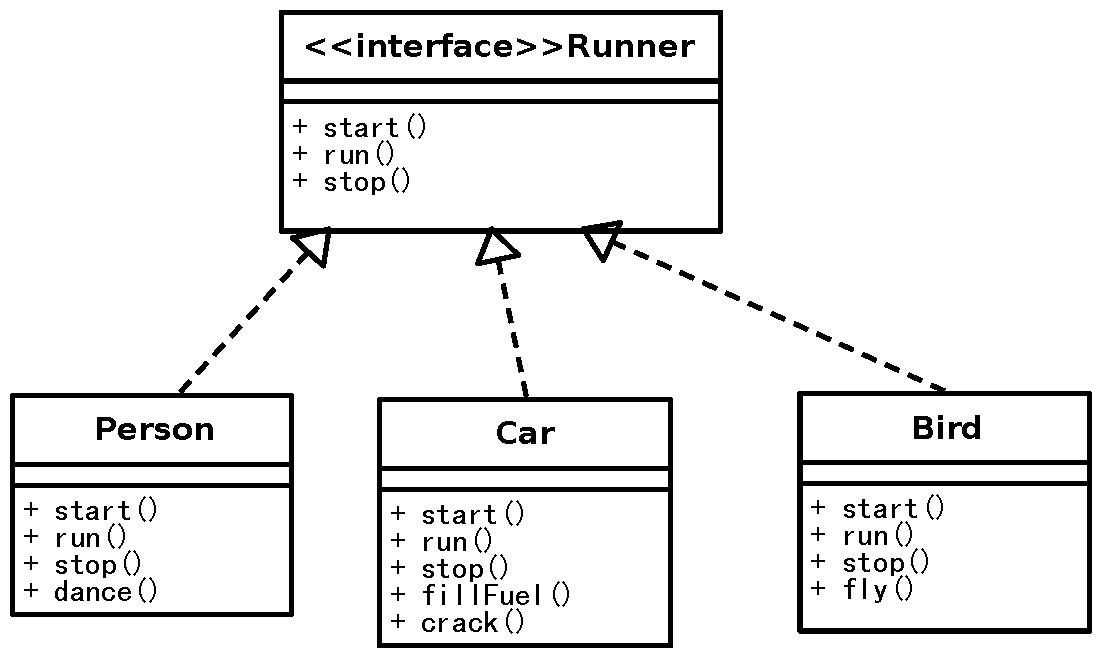
\includegraphics[width=0.8\textwidth]{a.pdf}
\end{figure}

通过接口可以指明多个类需要实现的方法,而这些类还可以根据需要继承各自的父类。或者
说,{\Mage 通过接口可以实现不相关类的相同行为,而不需要考虑这些类之间的层次关系。}
\end{frame}

\begin{frame}[fragile] % [fragile]参数使得能够插入代码
\frametitle{接口的多重实现}
\begin{javaCode}
interface Runner {
  public void run();
}
\end{javaCode}

\begin{javaCode}
interface Swimmer {
  public void swim();
}
\end{javaCode}
\begin{javaCode}
abstract class Animal {
  public abstract void eat();
}
\end{javaCode}
\begin{javaCode}
class Person extends Animal implements Runner, Swimmer {
  public void run() {
    System.out.println("I am running, to the sea!");
  }
  public void swim() {
    System.out.println("I am swimming, to the island!");
  }
  public void eat() {
    System.out.println("I am eating!");
  }
}
\end{javaCode}
\end{frame}

\begin{frame}[fragile] % [fragile]参数使得能够插入代码
\frametitle{接口的多重实现}
\begin{javaCode}
public class Test {
  public static void main(String args[]) {
    Test t = new Test();
    Person p = new Person();
    t.m1(p);
    t.m2(p);
    t.m3(p);
  }
  public void m1(Runner f) {
    f.run();
  }
  public void m2(Swimmer s) {
    s.swim();
  }
  public void m3(Animal a) {
    a.eat();
  }
}
\end{javaCode}
\end{frame}

\begin{frame}[fragile] % [fragile]参数使得能够插入代码
\frametitle{接口间的继承}

与接口的多重实现情况类似,由于不担心方法追溯调用上的不确定性,接口之间的继承允许“多重继
承”的情况。
\begin{javaCode}
interface A {
  public void ma();
}
interface B {
  public int mb(int i);
}
interface C extends A,B {  //接口的多重继承
  public String mc();
}
class D implements C {
  public void ma() {
    System.out.println("Implements method ma()!");
  }
  public int mb(int i) {
    return 2000 + i;
  }
  public String mc() {
    return "Hello!";
  }
}
\end{javaCode}
{\footnotesize \Mage 上述代码中的D类缺省继承了Object类,直接实现了接口C,间接实现了接口A和B,由于多态性的机
制,将来D类的对象可以当作Object、C、A或B等类型使用。}
\end{frame}

\begin{frame}[fragile] % [fragile]参数使得能够插入代码
\frametitle{接口特性总结}
\begin{itemize}
\item 通过接口可以实现不相关类的相同行为,而不需要考虑这些类之间的层次关系;
\item 接口可以被多重实现;
\item 接口可以继承其它的接口,并添加新的属性和抽象方法,接口间支持多重继承。
\end{itemize}
\end{frame}

\begin{frame}[fragile] % [fragile]参数使得能够插入代码
\frametitle{练习}
定义自己的接口、实现类和测试程序,体会接口的功能和用法。
\end{frame}

%%%%%%%%%%%%%%%%%%%%%%%%%%%%%%%%%%%%%%%%%%%%%%%%
\section{嵌套类}
\begin{frame}[fragile] % [fragile]参数使得能够插入代码
\frametitle{嵌套类}
Java语言支持类的嵌套定义,即允许将一个类定义在其他类的内部,其中内层的类被称为嵌套类
(Nested Class)。嵌套类可以分为两种:
\begin{description}
\item[静态嵌套类(Static Nested Class)] 使用static修饰的嵌套类;
\item[内部类(Inner Class)] 非static的嵌套类。
\end{description}
\begin{javaCode}
public class A {
  ...
  private class B {
    ...
  }
  public static class C {
    ...
  }
}
\end{javaCode}
\end{frame}

\begin{frame}[fragile] % [fragile]参数使得能够插入代码
\frametitle{内部类}
内部类又可分为三种情况:
\begin{enumerate}
\item {\hei 普通的内部类:}在Java类中,方法或语句块的外部定义的非static类。
\item {\hei 局部内部类:}也称局部类(Local Class),定义在方法或语句块中的类。
\item {\hei 匿名内部类:}也称匿名类(AnonymousClass),定义在方法或语句块中,该类没有名字、只能
  在其所在之处使用一次。
\end{enumerate}
\end{frame}

\begin{frame}[fragile] % [fragile]参数使得能够插入代码
\frametitle{内部类}
\begin{enumerate}
\item 内部类与其所在的外层类之间存在着逻辑上的依赖关系——内部类的对象不能单独存在,它必须依赖一
个其外层类的对象;
\item 在内部类中可以直接访问其外层类中的成员、包括属性和方法,即使这些属性和方法是private的。
\item 内部类可以声明为抽象类,因此可以被其它的内部类继承。也可以声明为final的。
\item 和外层类不同,内部类可以声明为private或protected。
\end{enumerate}
\end{frame}

\begin{frame}[fragile] % [fragile]参数使得能够插入代码
\frametitle{使用内部类\ding{182}}

\refcode{JavaSE\_03/TestInnerClass.java}

\samp{TestInner.java}
\begin{javaCode}
class A {
  private int s;
  public class B {
    public void mb() {
      s = 100;
      System.out.println("在内部类 B 中 s=" + s);
    }
  }
  public void ma() {
    B i = new B();
    i.mb();
  }
}

public class TestInner {
  public static void main(String args[]) {
    A o = new A();
    o.ma();
  }
}
\end{javaCode}

{\small \Mage 上述程序编译后生成三个文件:TestInner.class, A.class, A\$B.class。}
\end{frame}

\begin{frame}[fragile] % [fragile]参数使得能够插入代码
\frametitle{使用内部类\ding{182}}

\wxd{TestInner.java运行时的内存状态}

系统创建一个外层类的对象o,并将其实例变量s缺省初始化为0。

\begin{figure}
\centering
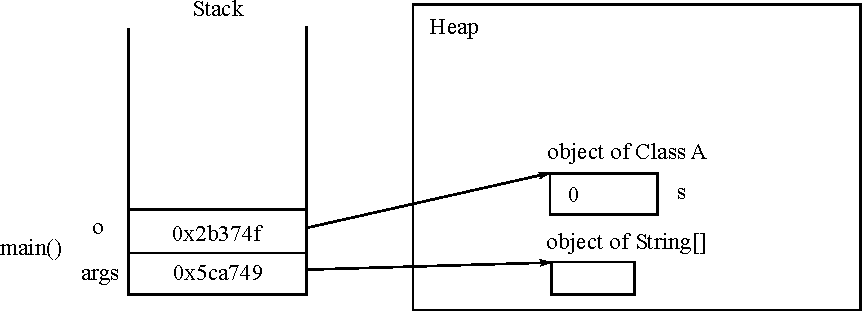
\includegraphics[width=0.8\textwidth]{innerclass01.pdf}
\end{figure}

\end{frame}

\begin{frame}[fragile] % [fragile]参数使得能够插入代码
\frametitle{使用内部类\ding{182}}

\wxd{TestInner.java运行时的内存状态}

调用对象o的成员方法ma(),首先为引用变量this分配空间以记录该方法本次运行时的当前对象,然后执行方法体中的第一条语句创建一个内部类B的对象i。

\begin{figure}
\centering
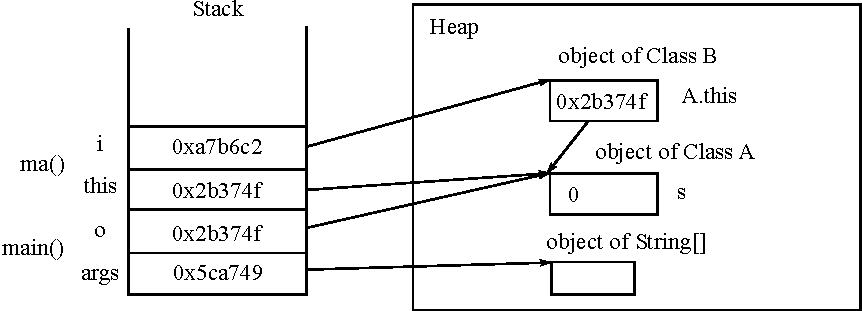
\includegraphics[width=0.8\textwidth]{innerclass02.pdf}
\end{figure}

{\kai\small 此时,内部类B中虽然未显式的定义任何属性,但其对象i一经创建,即拥有一个系统自动添加的属性(实例变量),该属性的数据类型为外层类对象的句柄,该属性为只读,且可以使用约定标记<外层类名>.this访问。}

\end{frame}

\begin{frame}[fragile] % [fragile]参数使得能够插入代码
\frametitle{使用内部类\ding{182}}

\wxd{TestInner.java运行时的内存状态}

内部类对象i调用其成员方法mb()。

\begin{figure}
\centering
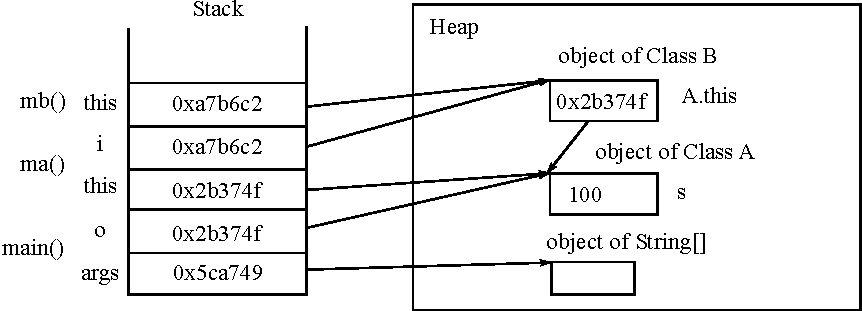
\includegraphics[width=0.8\textwidth]{innerclass03.pdf}
\end{figure}

{\kai\small 在方法体中遇到变量s时,按照如下处理过程:首先在当前方法mb()中检索是否存在局部变量(包括方法形参)s,没有则继续查找方法的当前对象(内部类B中)是否存在成员变量s,没有则通过属性A.this检索当前对象所依赖的外层类对象,最终找到并操作该变量s并赋值为100。}
\end{frame}

\begin{frame}[fragile] % [fragile]参数使得能够插入代码
\frametitle{使用内部类\ding{183}}

在外部使用其他类中的内部类虽然不提倡,但也是允许的。此时,应指明其完整层次,并显式建立对
象间的依赖关系。

\samp{A.java}
\begin{javaCode}
public class A {
  private int s;
  public class B {
    public void mb() {
      System.out.println(s);
    }
  }
}
\end{javaCode}
\samp{TestInner2.java}
\begin{javaCode}
public class TestInner2 {
  public static void main(String[] args) {
    A a = new A();
    // 创建一个依赖于 a 而存在的 b
    A.B b = a.new B();
    b.mb();
  }
}
\end{javaCode}
\end{frame}

\begin{frame}[fragile] % [fragile]参数使得能够插入代码
\frametitle{使用内部类\ding{184}}

内部类中出现变量命名冲突时,可以使用内部类对象的特殊属性“<外层类名>.this”来访问其所依赖
外层类对象的成员。
\samp{TestInner3.class}
\begin{javaCode}
class A {
  private int s = 111;
  public class B {
    private int s = 222;
    public void mb(int s) {
      System.out.println(s);  // 局部变量 s
      System.out.println(this.s);  // 内部类对象的属性 s
      System.out.println(A.this.s); // 外层类对象属性 s
    }
  }
}

public class TestInner3 {
  public static void main(String args[]) {
    A a = new A();
    A.B b = a.new B();
    b.mb(333);
  }
}
\end{javaCode}
{\small\Mage 输出结果为:333\textbackslash n 222\textbackslash n 111}
\end{frame}

\begin{frame}[fragile] % [fragile]参数使得能够插入代码
\frametitle{局部内部类}

局部内部类是定义在Java方法或语句块中的类型,相当于方法中的局部变量,其作用域仅限于其所在的方法体或者语句块。

\begin{itemize}\kai
\item 局部类声明时不允许加public、private等访问控制修饰符。
\item 局部类也不允许定义static属性和方法,{\Red 除非局部类为静态类(后续讲述)}。
\item 局部类中不但可以访问其所在外层类的成员,还可以访问其所在方法/语句块中的局部变量,但
  这些变量必须声明为{\Red final}。
\end{itemize}

\refcode{JavaSE\_03/TestLocalInnerClass.java}

{\hei\Red 不建议使用局部类。}
\end{frame}

\begin{frame}[fragile] % [fragile]参数使得能够插入代码
\frametitle{匿名内部类}
匿名内部类可以被认为是局部类的一种简化。

{\kai 当我们只在一处使用到某个类型时,可以将之定义为局部类,进而如果我们只是创建并使用该类的一
个实例的话,那么连类的名字都可以省略。}
\end{frame}

\begin{frame}[fragile] % [fragile]参数使得能够插入代码
\frametitle{使用匿名内部类\ding{182}}

\refcode{JavaSE\_03/TestAnonymousInnerClass.java}

\samp{Person.java}
\begin{javaCode}
public abstract class Person {
  private String name;
  private int age;
  public Person() {}
  public Person(String name, int age) {
    this.name = name;
    this.age = age;
  }
  public String getInfo() {
    return "Name: " + name + "\t Age: " + age;
  }
  public abstract void work();
}  
\end{javaCode}
\end{frame}

\begin{frame}[fragile] % [fragile]参数使得能够插入代码
\frametitle{使用匿名内部类\ding{182}}

\samp{TestAnonymous.java}
\begin{javaCode}
public class TestAnonymous {
  public static void main(String[] args) {
    Person sp = new Person() { \\ 匿名内部类
      public void work() {
        System.out.println("个人信息:" + this.getInfo());
        System.out.println("I am sailing.");
      }
    };
    sp.work();
  }
}
\end{javaCode}

\xyy{上述代码的解释}

{\small
定义一个新的Java内部类,该类本身没有名字,但继承了指定的父类Person,并在此匿名子类中重写
了父类的work()方法,然后立即创建了一个该匿名子类的对象,再将其句柄保存到引用变量sp中待
用。}
\end{frame}

\begin{frame}[fragile] % [fragile]参数使得能够插入代码
\frametitle{使用匿名内部类\ding{182}}

由于匿名类没有类名,而构造方法必须与类同名,所以{\hei 匿名类不能显式的定义构造方
  法}\pno{188},但系统允许在创建匿名类对象时将参数传给父类构造方法(使用父类的构造方法)。

\begin{javaCode}
Person sp = new Person("Kevin", 30) {
  public void work() {
    System.out.println("个人信息:" + this.getInfo());
    System.out.println("I am sailing.");
  }
};
\end{javaCode}
\end{frame}

\begin{frame}[fragile] % [fragile]参数使得能够插入代码
\frametitle{使用匿名内部类\ding{183}}

匿名类除了可以继承现有父类之外,还可以实现接口,但不允许实现多个接口,且实现接口时就不能
再继承父类了,反之亦然。

\refcode{JavaSE\_03/TestAnonymousInnerClass02.java}

\samp{Swimmer.java}
\begin{javaCode}
public interface Swimmer {
  public abstract void swim();
}
\end{javaCode}

\samp{TestAnonymous2.java}
\begin{javaCode}
public class TestAnonymous2 {
  public static void main(String[] args) {
    TestAnonymous2 ta = new TestAnonymous2();
    ta.test(new Swimmer() { // 匿名类实现接口
      public void swim() {
        System.out.println("I am swimming.");
      }
    });
  
  public void test(Swimmer swimmer) {
    swimmer.swim();
  }
}
\end{javaCode}
\end{frame}

\begin{frame}[fragile] % [fragile]参数使得能够插入代码
\frametitle{使用匿名内部类\ding{183}}

上述程序main()方法中的代码相当于:

\begin{javaCode}
public static void main(String[] args) {
  TestAnonymous2 ta = new TestAnonymous2();
  class Person implements Swimmer {
    public void swim() {
      System.out.println("I am swimming.")
    }
  }
  ta.test(new Person());
}
\end{javaCode}
\end{frame}

\begin{frame}[fragile] % [fragile]参数使得能够插入代码
\frametitle{静态嵌套类}

{\hei 静态嵌套类不再依赖/引用外层类的特定对象,只是隐藏在另一个类中而已。}

由于静态嵌套类的对象不依赖外层类的对象而独立存在,因而可以直接创建,进而也就无法在静态嵌
套类中直接使用其外层类的非static成员。
\begin{javaCode}
class A {
  public static int total = 0;
  public static class B {
    public void mb() {
      total = 100;
      System.out.println(total);
    }
  }
}  

public class TestStaticNestedClass {
  public static void main(String[] args) {
    A.B b = new A.B();
    b.mb();
  }
}
\end{javaCode}
\end{frame}

\section{枚举类型}
\begin{frame}[fragile] % [fragile]参数使得能够插入代码
\frametitle{枚举类型}

{\hei Java SE 5.0开始,引入了一种新的引用数据结构——枚举(Enum)。}

{\kai Java语言中枚举类型均自动继承了java.lang.Enum类(该类继承自Object类)。枚举类型使用一组常
量值来表示特定的数据集合,该集合中数据的数目确定(通常较少),且这些数据只能取预先定义的
值。}

\begin{javaCode}
public enum Week {
  MON, TUE, WED, THU, FRI, SAT, SUN
}
\end{javaCode}

\wxd{之前我们如何解决上述需求?}

之前实现枚举类的功能,Java开发者一般采用声明多个整型常量的做法。

\begin{javaCode}
public class Week {
  public static final int MON = 1;
  public static final int TUE = 2;
  ...
}    
\end{javaCode}
\end{frame}

\begin{frame}[fragile] % [fragile]参数使得能够插入代码
\frametitle{使用枚举类型}
\begin{javaCode}
public enum Week {
  MON, TUE, WED, THU, FRI, SAT, SUN
}  
\end{javaCode}
\begin{javaCode}
public class TestEnum {
  public static void main(String[] args) {
    TestEnum te = new TestEnum();
    te.work(Week.SUN);
  }
  public void work(Week day) {
    if (day.equals(Week.SAT)) {
      System.out.println("购物!");
    }else if (day.equals(Week.SUN)) {
      System.out.println("祈祷!");
    } else {
      System.out.println("工作!");
    }
  }
}
\end{javaCode}
\end{frame}

\begin{frame}[fragile] % [fragile]参数使得能够插入代码
\frametitle{遍历枚举类型常量值}

可以使用静态方法values()遍历枚举类型常量值。

\samp{ListEnum.java}
\begin{javaCode}
public class ListEnum {
  public static void main(String[] args) {
    Week[] days = Week.values();
    for(Week d: days) {
      System.out.println(d);
    }
  }
}
\end{javaCode}
\end{frame}

\begin{frame}[fragile] % [fragile]参数使得能够插入代码
\frametitle{组合使用枚举类型与switch}

使用枚举类型通常是为了实现多路分支性结构。

\begin{javaCode}
public class TestEnumInSwitch {
  public static void main(String[] args) {
    TestEnumInSwitch teis = new TestEnumInSwitch();
    teis.work(Week.FRI);
  }
  public void work(Week day) {
    switch(day) {
      case MON:
      case TUE:
      case WED:
      case THU:
      case FRI:
        System.out.println("工作日,去上班!");
        break;
      case SAT:
        System.out.println("星期六,去购物!");
        break;
      case SUN:
        System.out.println("礼拜天,去教堂!");
        break;
      default:
        System.out.println("你有没有搞错!");
    }
  }
}
\end{javaCode}
\end{frame}

\begin{frame}[fragile] % [fragile]参数使得能够插入代码
\frametitle{组合使用枚举类型与switch}

\wxd{注意}
\begin{enumerate}
\item case字句必须省略其枚举类型的前缀,即只需要写成 case SUN:,而不允许写成 case
  Week.SUN:,否则编译出错。
\item 不必担心系统无法搞清这些常量名称的出处,因为switch后的小括号中的表达式已经指明本次
  要区分处理的是Week类型常量。
\end{enumerate}


\end{frame}
%%%%%%%%%%%%%%%%%%%%%%%%%%
% \begin{frame}[fragile] % [fragile]参数使得能够插入代码
% \frametitle{}
% 
% \end{frame}
%%%%%%%%%%%%%%%%%%%%%%%%%%
%% \begin{frame}
%% \frametitle{本章习题}
%% \begin{enumerate}
%% \item a
%% \item b
%% \end{enumerate}
%% \end{frame}

%% \begin{figure}
%% \centering
%% 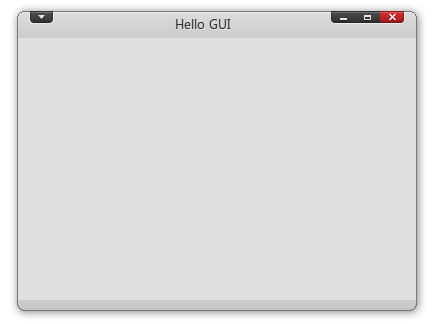
\includegraphics[width=0.6\textwidth]{fig01.png}
%% \end{figure}
% TKS %%%%%%%%%%%%%%%%%%%%%%%%%%%%%%%%%%%%%%%%%%%%%%
\begin{frame}
\centering
{\Huge \textcolor{blue}{THE END}} \\
\vspace{5mm}
{\Large wxd2870@163.com} \\
\end{frame}
%%%%%%%%%%%%%%%%%%%%%%%%%%%%%%%%%%%%%%%%%%%%%%%%%%
\end{document}
